\def\ktitle{FPGA ASSIGNMENT}
\def\kauthor{Koushik Kalyani}
\def\kcontact{koushikkalyani369@gmail.com}
\def\kmodule{IITH - Future Wireless Communication}
\documentclass[journal,12pt,twocolumn]{IEEEtran}
\usepackage{enumitem}
\usepackage{tikz}
\usepackage{circuitikz}
\usepackage{karnaugh-map}
\usepackage{tabularx}
\usepackage{circuitikz}
\usepackage{tikz}
\usepackage{titlesec}
\usepackage{multicol}
\title{\ktitle}
\author{\kauthor\\\kcontact\\\kmodule}
\begin{document}
\maketitle
\tableofcontents
\section{\textbf{Question}}
In the circuit shown below, X and Y are digital inputs, and Z is a digital output. The equivalent circuit is a\\
\\\resizebox{0.45\textwidth}{!}{
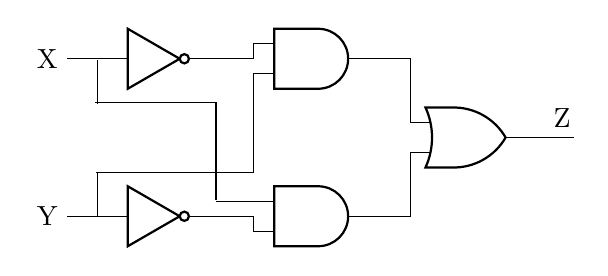
\begin{tikzpicture}
	\ctikzset{
		logic ports=ieee,
		logic ports/scale=0.68,
		logic ports/fill=white}
	\node[not port](x) at (0,0){};
	\node[not port](y) at (0,-2){};
	\node[and port](a) at (2,0){};
        \node[and port](b) at (2,-2){};
        \node[or port](c) at (4,-1){};
	\draw(x.out)-|(a.in 1);
	\draw(y.out)-|(b.in 2);
        \draw(a.out)-|(c.in 1);
        \draw(b.out)-|(c.in 2);
	\draw(a.in 2)|- ++(-2,-1.25) ;
        \draw(-0.72,-1.45)-- ++(0,-0.55);
        \draw(0.79,-1.8)|- ++(-1.53,1.25) ;
        \draw(b.in 1)-- ++(-.48,0);        
        \draw(-0.72,-.019)-- ++(0,-0.55);
	\draw(y.in 1)-- ++(-0.5,0) node[left]{Y};
        \draw(x.in 1)-- ++(-0.5,0) node[left]{X};
	%\draw(b.in 2)-- ++(-4.5,0) node[left]{S};
	\draw(c.out)-- ++(0.6,0) node[near end,above]{Z};
\end{tikzpicture}
}

\begin{multicols}{2}
\begin{enumerate}[label=(\Alph*)]
	\item NAND gate
	\item NOR gate
	\item XOR gate
	\item XNOR gate 
\end{enumerate}
\end{multicols}
\section{\textbf{Answer}}
The above question can be solved as $X\cdot \bar Y + \bar X \cdot Y$ .i.e equivalent circuit is XOR-circuit.\\
\section{\textbf{K-Map Implementation}}
\resizebox{0.45\textwidth}{!}{%
	\begin{karnaugh-map}[2][2][1][X][Y]
		\maxterms{0,3}
		\minterms{1,2}
            \implicant{1}{1}
             \implicant{2}{2}
	\end{karnaugh-map}%
}
\centering
Therefore $Z=X\cdot \bar Y + \bar X \cdot Y$
\section{\textbf{Truth Table}}
\begin{tabularx}{0.45\textwidth}{
  | >{\centering\arraybackslash}X  
  | >{\centering\arraybackslash}X 
  | >{\centering\arraybackslash}X |
  }
  \hline
  \textbf{$X$}&\textbf{$Y$}&\textbf{$Z$}\\
  \hline
  0&0&0\\
  \hline
  0&1&1\\
  \hline
  1&0&1\\
  \hline
  1&1&0\\
  \hline
  \end{tabularx}
\begin{center} 
 Truth table for Boolean funtion $Z$
\end{center}
\section{\textbf{Logic Diagram}}
\resizebox{0.45\textwidth}{!}{
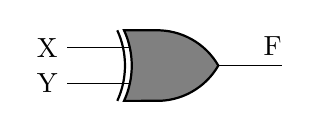
\begin{tikzpicture}
	\ctikzset{
		logic ports=ieee,
		logic ports/scale=0.8,
		logic ports/fill=gray}
	\node[xor port](xor) at (0,0){};
	\draw(xor.in 1)-- ++(-0.5,0) node[left]{X};
	\draw(xor.in 2)-- ++(-0.5,0) node[left]{Y};
	\draw(xor.out)-- ++(0.5,0) node[near end,above]{F};
\end{tikzpicture}
}
\begin{center}
	Fig. 2
\end{center}
	\section{\textbf{Components}}
	\begin{tabularx}{0.45\textwidth}{
			| >{\centering\arraybackslash}X
			| >{\centering\arraybackslash}X
			| >{\centering\arraybackslash}X |
			}
			\hline
			\textbf{Components}&\textbf{Values}&\textbf{Quantity}\\
			\hline
			VAMAN & FPGA & 1\\
			\hline
			Jumper Wires & F-M & 6\\
			\hline
			Breadboard & & 1\\
			\hline
               LED &&1\\
               \hline
               Resistor&$\leq$ 220 Ohms&1\\
               \hline
	\end{tabularx}
\section{\textbf{Implementation}}
\begin{tabularx}{0.45\textwidth}{
		| >{\centering\arraybackslash}X
		| >{\centering\arraybackslash}X
		| >{\centering\arraybackslash}X|}
\hline
	\textbf{VAMAN PIN}&\textbf{INPUT}&\textbf{OUTPUT}\\
	\hline
	21&X& \\
	\hline
	22&Y&\\
	\hline
	18&&F\\
	\hline
\end{tabularx}\\
\centering
Connections\\
\textbf{Procedure}
\begin{enumerate}[label={\arabic*}.]
	\item Connect the circuit as per the above table.
	\item Connect inputs to Vcc for Logic 1, ground for Logic 0.
	\item Execute the circuit using the below codes.\\
		\vspace{\baselineskip}
		   \begin{tabularx}{0.45\textwidth}{
				| >{\centering\arraybackslash}X|}
			\hline
                  https://github.com/koushikkalyani/FWC/blob\\/main/FPGA/helloworldfpa.v\\
			\hline
		\end{tabularx}\\
	    \vspace{\baselineskip}
	\item Change the values of $X,Y$ in the Hardware and verify the Truth Table.
\end{enumerate}
 \textbf{How to execute}
 \begin{enumerate}[label={\arabic*}.]
 \item Write your code in helloworldfpga.v file.
 \item Also update .pcf file for pin configuration.
 \item To compile use the below command by changing directory appropriately.\\
 ql\_symbiflow -compile -src /data/data/com.termux/files/home/fpga-examples/blink -d ql-eos-s3 -P PU64 -v helloworldfpga.v -t helloworldfpga -p quickfeather.pcf -dump binary.
 \item Connect your mobile hotspot to laptop and send .bin file by using command.\\
 scp /data/data/com.termux/files/home/fpga-examples/blink/helloworldfpga.bin pi@192.168.0.114:\\
 change pi as your system name and IP address. 
 \item If you dont have Tinyfpga then type the following command.\\
 git clone --recursive https://github.com/QuickLogic-Corp/TinyFPGA-Programmer-Application.git\\
 sudo pip3 install tinyfpgab pyserial\\
 sudo reboot\\
 \item Connect the Vaman to the Raspberry Pi through USB.
 \item There is a button and an LED to the left of the USB port on the Vaman.  There is another button to the right of teh LED.
 \item Press the right button first and immediately press the left button.  The LED will be blinking green.  The Vaman is now in bootloader mode.
 \item  Then execute the following.\\
 python3 /home/pi/TinyFPGA-Programmer-Application/tinyfpga-programmer-gui.py --port /dev/ttyACM0 --appfpga /home/pi/helloworldfpga.bin --mode fpga --reset\\
 Suitably change pi as your system name.
 \end{enumerate}
\end{document}g
